\documentclass[11pt,english]{article}
\usepackage[T1]{fontenc}
\usepackage{fullpage}
\usepackage{babel}
\usepackage{graphicx}
\usepackage{amssymb}
\usepackage{amsmath}

\begin{document}

\title{\bf COMP4106 -- Assignment 3}
\author{Brandon Schurman, 100857068}
\date{March 30, 2015}
\maketitle


\section{Classifying Independent Variables}
To classify a binary vector of independent variables, we implement an optimal Bayesian Classification algorithm. 
In this system, we use the Bayesian Classifier to place a vector $x$ into one of the four classes $\omega_1, ..., \omega_4$.
The true values of the four classes are randomly generated by the system in a preprocessing phase. 
Each class is represented as vector of $d=10$
features, where each of the $d$ features are randomly and independently (of the other nine
features) assigned a probability 
value in the range of $0$ tot $1$. 
The system uses these classes to randomly generate samples of $2,000$ binary vectors. A
binary sample vector contains $d$ indices, 
where each index is assigned a $1$ or instead a $0$ with the probability defined in feature $i$ of the corresponding class.
\vspace{2mm}\\
After the system obtains a sample of $2,000$ binary vectors for each of the four classes, it then uses an 8-fold cross validation scheme 
for training and testing. Thus, $1,750$ of the samples are used to train the classification algorithm, while the remaining $250$ are used
next to test and record the accuracy of the classification. The true values of the four classes are unknown to the classifier during 
training and testing.
The training proceudre thus uses the given samples to estimate the true probabilities of each feature, for each of the four classes.
Next in the testing phase, the system classifies each sample vector $x$ into one of the
four estimated classes. It infers, using the bayesian classifier
$$\Pr(x\mid\omega_i)\lessgtr\Pr(x\mid\omega_j)$$ pairwise for each of the four classes, wich class has the highest probability of containing the vector $x$. More specifically, the
probability of $x$ being a vector from a class $\omega_j$ is calculated as
$$\Pr(x\mid\omega_j) = \prod_{i=1}^{d}\Pr(x_i\mid\omega_j)$$
After testing the classifier with $250$ samples, we conclude that the classification is accurate to a degree of about $85\%$ on average. 
We also notice that there are some edge cases where the sample space is significantly less accurate, to a degree of $50\%$ or less, while other sample spaces may be classified with up to $100\%$ accuracy. Since the system randomly generates the true classes, it is indeed possible that some 
class instances may have a set of features where each feature has a value of nearly $0.5$,
making the classification inherently difficult. Likewise, if the features in a class
happen to be closer to $0.0$ or $1.0$, the classification is inherently much easier and
thus much more accurate. Furthermore, increasing the sample size from $2,000$ to $20,000$
or even $200,000$ was tested and did not appear to affect the accuracy of the classification 
in any significant way. When testing with the provided example datasets, the
classification was in fact innacurate, classifying only about $12\%$ of vectors correctly.

\pagebreak
\section{Classifying Variables Using a Dependence Tree}
To classify a binary vector of dependent variables, we must also infer a dependence tree to model the conditional probabilities of each 
feature $d_i$ for each of the four classes $\omega_1,...,\omega_4$. Like in the independence case, the system first randomly generates the 
true conditional probabilities for each of the four classes in a preprocessing phase. The classes all follow the same dependence relation, which 
has been hard-coded into the system. The actual dependence relation between the features is shown in \underline{Figure 2.1}. The system gnerates a random sample of $2,000$ binary vectors using the predefine dependence tree to train and test the classification.
\vspace{2mm}\\
Using an 8-fold cross-validation scheme for each of the four classes, the system using the first $1,750$ samples to estimate the true dependence tree. 
To estimate the tree, the Mutual Information is calculated on each edge between every pair of features in 
the entire given sample space of binary vectors. The Mutual Information of the feature $X$ relative to $Y$ is given by 
$$I(X;Y) = \sum_{x\in X}\sum_{y\in Y} p(x,y) \log \frac{p(x,y)}{p(x)\, p(y)}$$
Calculating the Mutual Information for every pair of features yields a set of weighted edges for a completely connected and undirected graph.
The systems can then run Kruskal's algorithm on this graph to solve for the maximum spanning tree, which is an estimate of the true dependence tree. An example of an estimated dependence tree obtained by the system can be found at \underline{Figure 2.2}. Next, the system uses the estimated depence tree structure to learn (i.e. estimate and store) the conditional probabilities of each feature.
Once the conditional probabilities are obtained, the system can now begin testing the classification with the remaining $250$ samples.
To determine which class
has the highest probability of producing the binary vector $x$, the classification algorithm uses a pairwise bayesian classifier
$$\Pr(x\mid\omega_i)\lessgtr\Pr(x\mid\omega_j)$$ where the conditional
probability that a vector $x$ is from class $\omega_j$ is calculated as
$$\Pr(x\mid\omega_j) = \Pr(x_r)\cdot\prod_{\substack{i=1\\ i\neq r}}^{d}\Pr(x_i\mid
x_{p(i)})$$
where $x_r$ is the root feature in the dependnce tree, and $x_{p(i)}$ is the parent of
the feature $x_i$ in the depence tree.
Through testing, We conclude that the classification of binary dependant variables is accurate to a degree of about $50\%$. 
This is significantly less accurate than that of the independence classifier. Again, increasing the sample size does not seem to affect
this accuracy. When testing with the provided example datasets, the
classification was in fact innacurate, classifying only about $12\%$ of vectors correctly.



\pagebreak
\underline{Figure 2.1: The true dependence tree}\\
\begin{center}
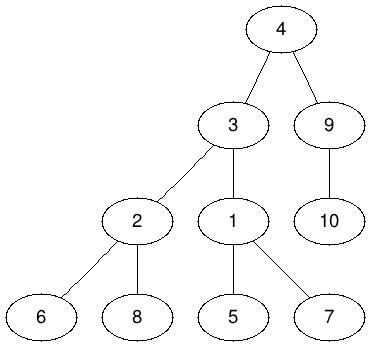
\includegraphics[width=3in]{tree.png} \\
\end{center}
\vspace{5mm}
\underline{Figure 2.2: An approximated dependence tree} \\
\begin{center}
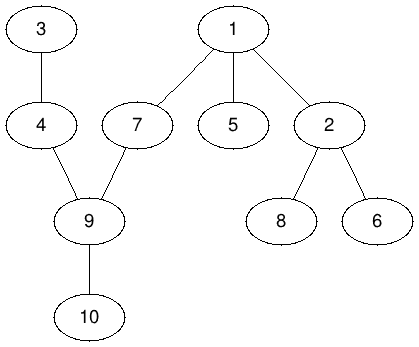
\includegraphics[width=3in]{est-tree.png}
\end{center}

\end{document}
